% !TEX root = ../om_ts_01.tex

\begin{frame} % название фрагмента

\videotitle{Компоненты ряда}

\end{frame}



\begin{frame}{Компоненты ряда: план}
  \begin{itemize}[<+->]
    \item Тренд, цикличность и сезонность.
    \item Аддитивное и мультипликативное разложение.
    \item Откуда взять формальное определение?
  \end{itemize}

\end{frame}


\begin{frame}{Умение видеть единорогов}

Аддитивное разложение ряда:
\[
y_t = trend_t + seas_t + remainder_t.
\]

\pause

\alert{Тренд} — плавно изменяющаяся составляющая ряда.

\pause

\alert{Сезонная составляющая} — составляющая с чёткой периодичностью и стабильной интенсивностью.

\pause

\alert{Случайная компонента} (остаток) — всё остальное. 

\end{frame}

\begin{frame}{Тренд, сезонность и остаток}

  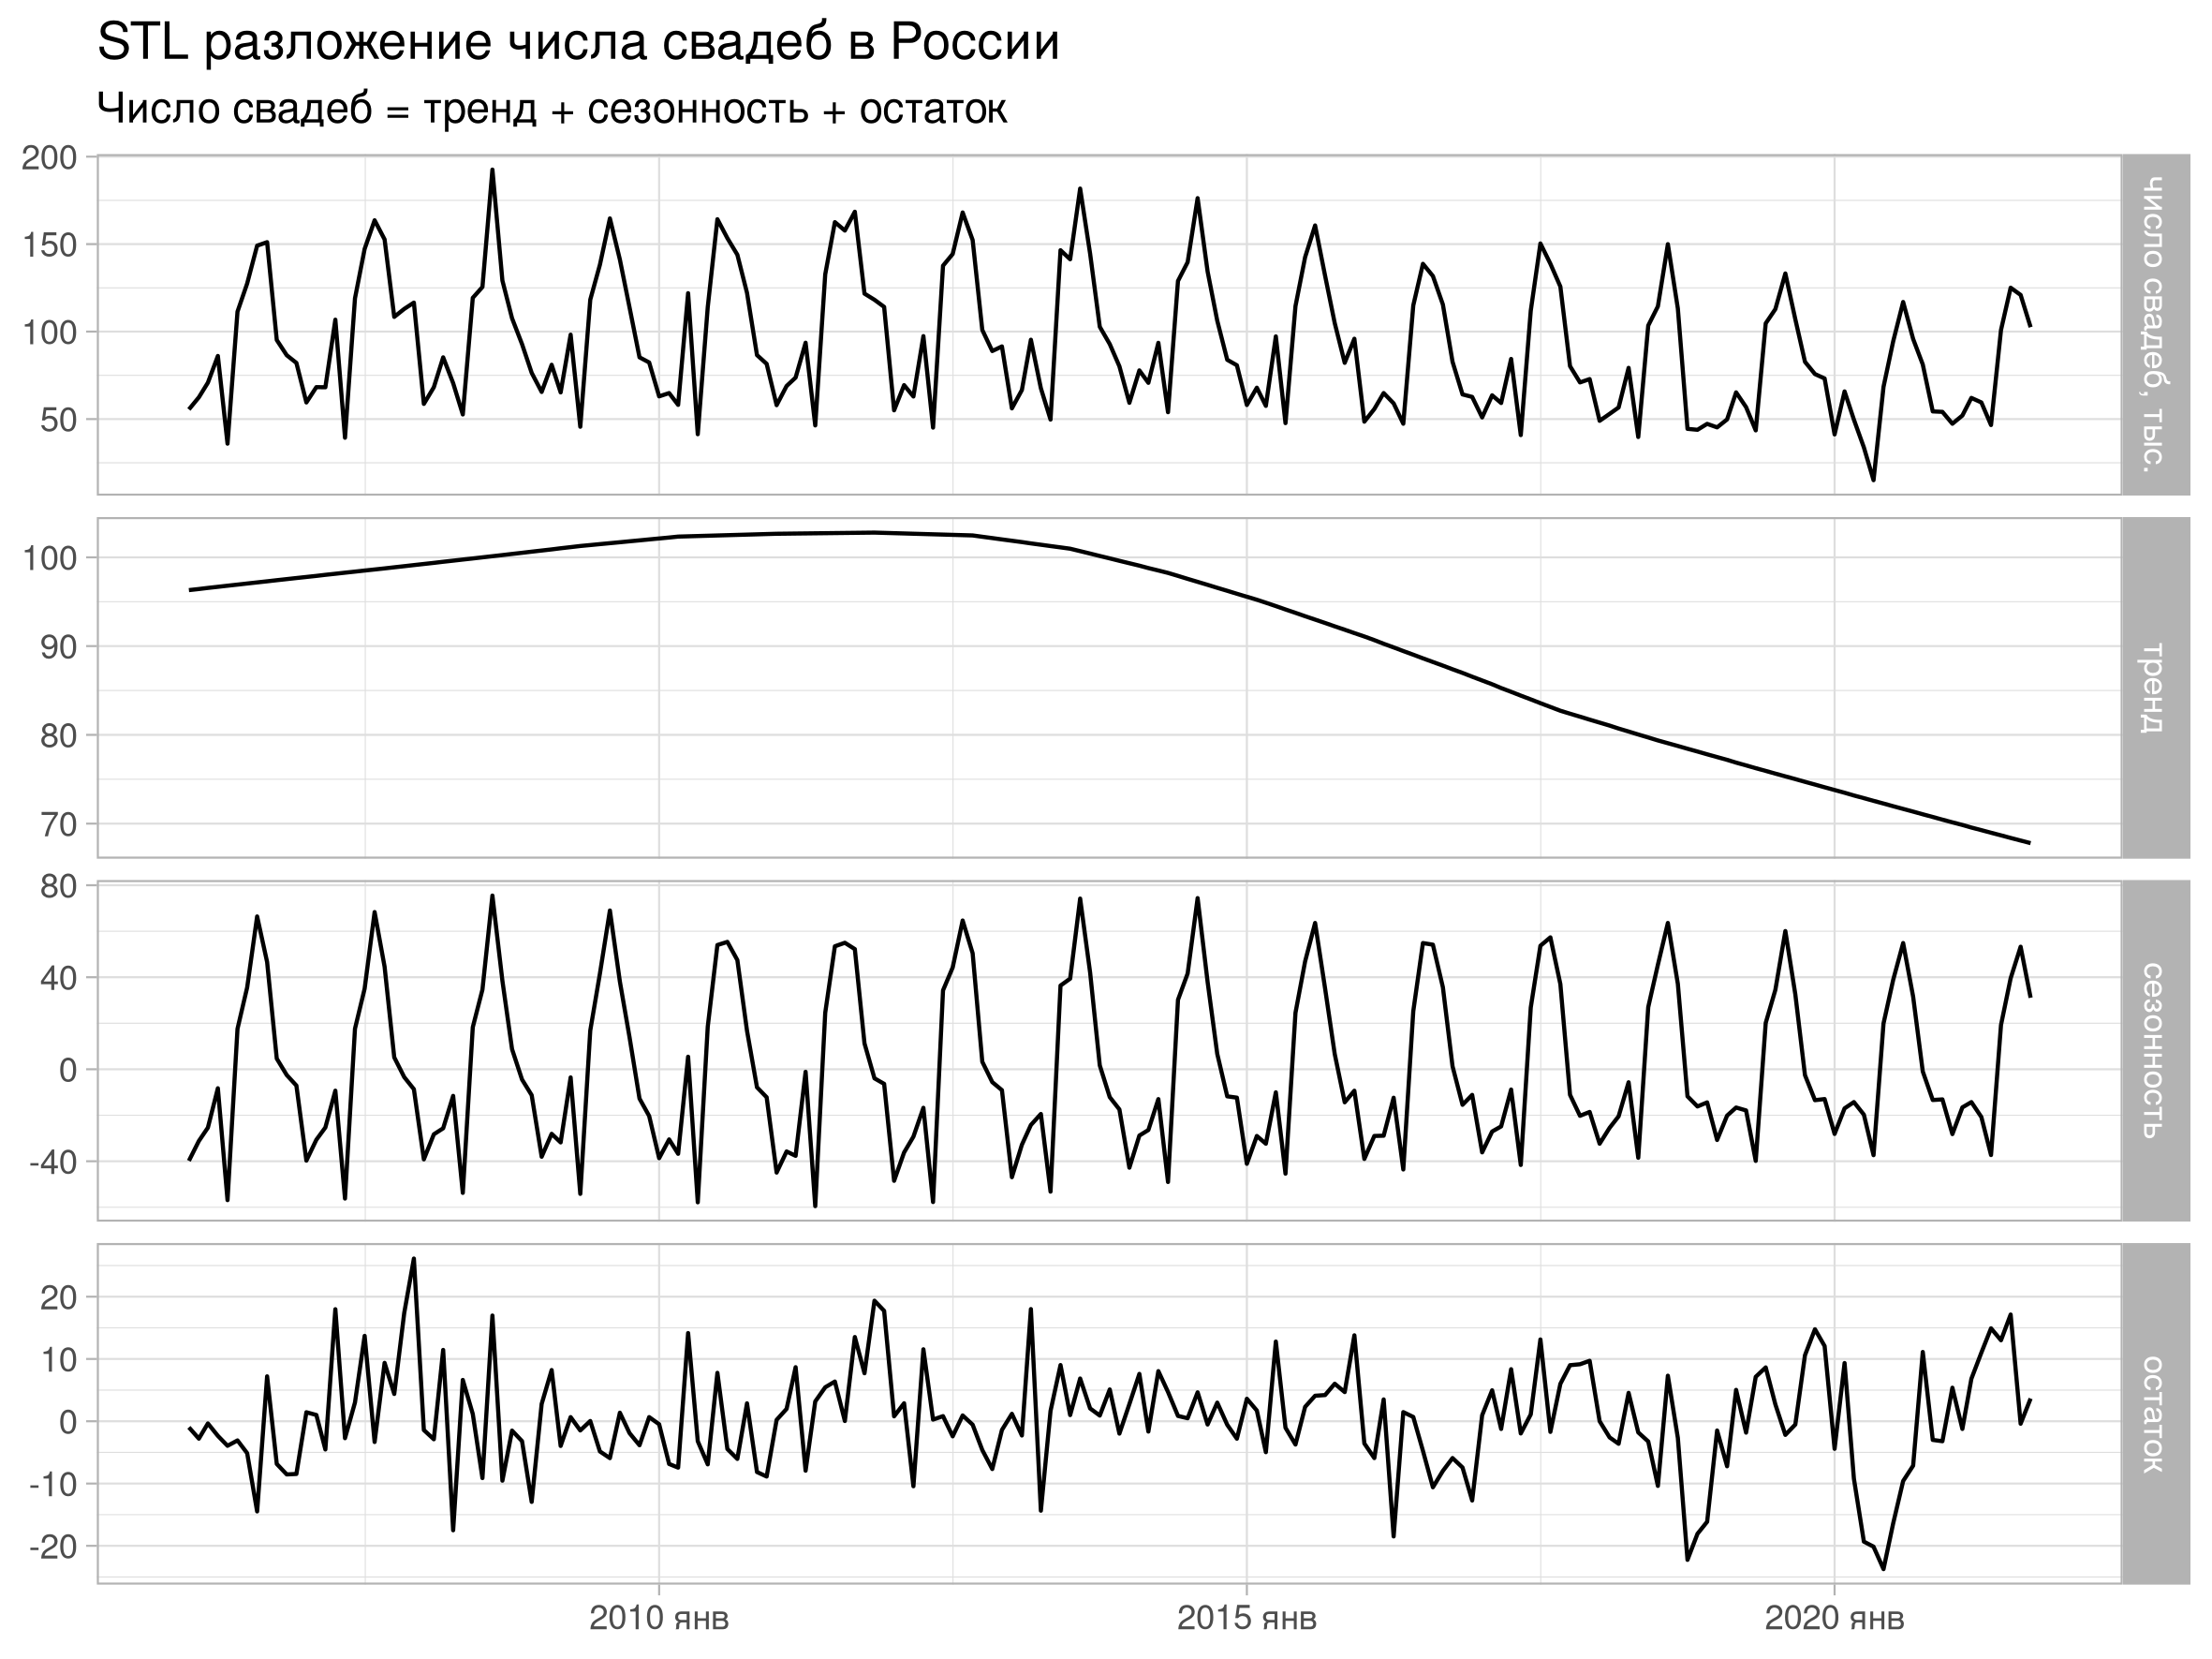
\includegraphics[width=\textwidth]{pictures/om_ts_01-041.png}

\end{frame}

\begin{frame}{Строгое определение?}

\pause
Единого строгого определения \alert{не} будет!

\pause
Некоторые модели и алгоритмы формально \alert{определяют} данные составляющие.

\end{frame}

\begin{frame}{Циклическая составляющая}

Иногда ряд раскладывают дальше
\[
y_t = trend_t + cycle_t + seas_t + remainder_t
\]

\pause
\alert{Циклическая составляющая} — составляющая с плавающей периодичностью и нестабильной интенсивностью. 


\pause
\alert{Тренд} (в узком смысле) —  плавно изменяющаяся монотонная составляющая ряда.

\end{frame}


\begin{frame}{Аддитивное и мультипликативное разложение}


\alert{Аддитивное} разложение ряда:
  \[
  y_t = trend_t + seas_t + remainder_t.
  \]
  
\pause
\alert{Мультипликативное} разложение ряда:
  \[
  y_t = trend_t \cdot seas_t \cdot remainder_t.
  \]

\pause
Превращаем одно в другое:
\[
  \ln y_t = \ln trend_t + \ln seas_t + \ln remainder_t.
\]
\end{frame}


\begin{frame}{Какие единороги лучше?}

Формальное определение составляющих \alert{зависит от модели}.

\pause
\alert{Алгоритм STL}: одно разложение $y_t = trend_t + seas_t + remainder_t$.

\pause
\alert{Модель ETS(AAA)}: другое разложение $y_t = trend_t + seas_t + remainder_t$.


\pause
Важно понимать \alert{цель построения} разложения. 

\end{frame}

\begin{frame}{А зачем разложение?}

  \begin{itemize}[<+->]
    \item Интересно \alert{само по себе}. 
    \item Для \alert{прогнозирования} ряда с помощью прогнозирования составляющих.
    \item Для получения \alert{характеристик ряда}. 
  \end{itemize}

  \pause
  А характеристики зачем?

  \begin{itemize}[<+->]
    \item Чтобы классифицировать новый ряд в один из заданных классов.
    \item Чтобы выявить в рядах неизвестные кластеры. 
  \end{itemize}
  
\end{frame}


\begin{frame}{Компоненты ряда: итоги}
  \begin{itemize}[<+->]
    \item Тренд \alert{плавно меняется} и включает цикличную составляющую.
    \item Сезонная составляющаю имеет \alert{чёткую периодичность} и \alert{стабильную амплитуду}.
    \item Точная формализация компонент \alert{зависит от модели}. 
  \end{itemize}

\end{frame}
